% !TeX root = ../my-thesis.tex
\chapter{Energieeffizientes Multithreading}
\section{Theoretische Einführung in die Parallelität}
Das Ziel hinter der Parallelisierung von Aufgaben ist die Beschleunigung der Laufzeit bei der Abarbeitung von Programmabläufen und die Minimierung der Wartezeiten des Prozessors. Solche Wartezeiten können entstehen, wenn während der Programmausführung Benutzereingaben nötig sind bevor die Ausführung fortgesetzt werden kann oder wenn neue Daten aus dem vergleichsweise langsamen Hauptspeicher nachgeladen werden müssen, da der prozessoreigene Cache nicht groß genug ist \cite[1135]{wolf2020}. Ohne Parallelität würden moderne Softwareanwendungen jeglicher Art nahezu unnutzbar werden. Einfache Vorgänge wie das Laden von Benutzerdaten aus einer lokalen Datenbank oder das downloaden von Bildern aus dem Netz, würden zum Einfrieren der Benutzeroberfläche führen, da bei sequentiellen Programmabläufen alle Aufgaben strikt hintereinander ausgeführt werden müssen. Android selbst wäre ohne Parallelität nicht umsetzbar, da Android's Architektur Multithreading und damit Parallelität voraussetzt.\todo{Erklärung}

Für die Realisierung von Parallelität haben sich mit der Evolution der Prozessortechnologie verschieden Ansätze und Techniken entwickelt. Jede dieser Techniken ist bis heute relevant und glänzt in unterschiedlichen Anwendungsfällen.

\underline{Pipelining}

Beim Pipelining wird die Ausführung von Befehlen in verschiedene Phasen aufgeteilt, welche jeweils durch eine eigene Ausführungseinheit bearbeitet werden. Sobald ein Befehl die aktuelle Phase abgeschlossen hat und zur nächsten Phase springt, kann bereits mit der Bearbeitung des nächsten Befehls, in der frei gewordenen Phase begonnen haben. In \autoref{fig:Pipeline} ist ein Beispiel einer 5-Phasen Pipeline veranschaulicht. Die Bearbeitung jeder Phase dauert im Optimalfall einen Taktzyklus, da andernfalls die Pipeline durch dies Phase geblockt werden kann, wie es in diesem Beispiel bei Befehl 3 während der Execute Phase der Fall ist. Ein großer Nachteil von Pipelining tritt bei häufigen Programmsprüngen auf, da bei jedem Sprung die komplette Pipeline geleert werden muss und alle Phasen, die bis dorthin vollendet wurden, verworfen werden und umsonst bearbeitet wurden. Dieser ist besonders bei größeren Pipelines kritisch \cite{pipelineElektro}.
\begin{figure}[H]
	\begin{center}	 
	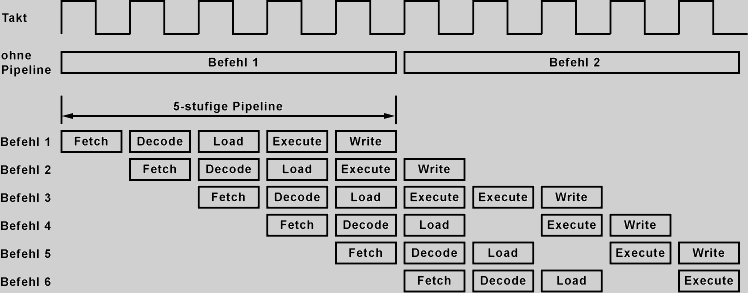
\includegraphics[scale=1]{Pipeline}
	\caption{Beispiel für eine 5-Phasen-Pipeline (Quelle: \cite{pipelineElektro})}
	\label{fig:Pipeline} 
	\end{center}
\end{figure}

\underline{simultanes Multi-Threading}

Ein Thread ist ein sequenzieller Ausführungspfaden innerhalb eines Prozesses, der ausgeführt wird. Bei Rechnern mit einem Prozessor kann zu einem Zeitpunkt immer nur ein Thread eines Prozesses gleichzeitig ausgeführt werde. Falls dieses Ausführung durch Ereignisse wie Speicherzugriffe oder Nutzereingaben warten muss, blockiert dieser Thread die \ac{cpu}. Durch sogenanntes simultanes Multi-Threading wird die verfügbare \ac{cpu} Zeit auf mehrere Prozesse und Threads aufgeteilt. Die \ac{cpu} kann dadurch zwischen den Threads hin und her springen und so längere Wartezeiten verhindern. Dies steigert die Effizienz der \ac{cpu} hinsichtlich der Laufzeit sowie des Energieverbrauchs \cite[877]{cplusplus}.

\underline{Hyper-Threading}

Die Technologie Hyperthreading wurde von Intel mit den Prozessoren Pentium 3, Pentium 4 und Xeon eingeführt. Hierbei wird wird der Durchsatz von Multithreaded-Anwendungen im Multitasking erhöht, indem sie die Auslastung der On-Chip-Ressourcen erhöht, die in der Intel-NetBurst-Mikroarchitektur verfügbar sind. Ein typischer Thread belastet nur etwa 35 \% der NetBurst-Ausführungsressourcen. Hyperthreading erhöht die Auslastung durch notwendige Logik und Ressourcen, die der CPU hinzugefügt werden. Für die Aufteilung der einkommenden Daten auf den freien Raum sorgen somit zwei logische Prozessoren, die vom Betriebssystem mittels klassischer Multiprocessing-Verfahren verwaltet werden \cite[1138]{wolf2020}. Somit stehen dem Rechner also 2 logische Rechenkern zur Verfügung trotz physischer Single Core \ac{cpu}. Dies bietet die Möglichkeit Speicherwartezeiten zu überbrücken. Wenn der erste Thread im Wartezustand ist, kann der Prozessor mithilfe des zweiten logischen Kerns in der Programmausführung fortfahren.

\underline{Multi-Core-Prozessor}

Bei Multi-Core Systemen handelt es sich um Prozessoren mit mehreren physischen Rechenkernen. Diese können voneinander unabhängig arbeiten und ermöglichen echte Parallelität. Alle Rechenkerne nutzen auch die schon genannten Techniken um möglichst effiziente Ergebnisse zu erhalten. Der Vorteil liegt hierbei nicht nur in der Steigerung der Geschwindigkeit. Mehrkernprozessoren können wesentlich geringer getaktet werden als Single Core Prozessoren und ermöglichen trotzdem erhöhte Laufzeitgeschwindigkeit bei geringerer Leistungsaufnahme und Wärmeentwicklung \cite{MulicoreElektro}. Es könnte die Annahme getroffen werden, dass mit steigender Rechenkernzahl auch die Leistung addiert wird. Sodass die neue Laufzeit im Multi-Core-Betrieb gleich der ursprünglichen Laufzeit mit einem Kern geteilt durch die Anzahl der Rechenkerne beträgt. In der Realität ist dies jedoch nicht umsetzbar, da verschiedene Faktoren diese Annahme begrenzen. Zunächst einmal wächst mit steigender Anzahl an Rechenkernen auch der Aufwand der Verwaltung durch das Betriebssystem. Außerdem ist es nicht einfach den Zugriff auf geteilte Speicherressourcen durch mehrere Rechenkerne zu synchronisieren. Die Laufzeit für parallele Prozesse setzt sich grob aus folgenden Anteilen zusammen.
\begin{aligneddescription}
\item[Rechenzeit] Zeit für die Durchführung von Berechnungen unter Verwendung von Daten im lokalen Speicher der einzelnen Prozessoren.
\item[Kommunikationszeit] Zeit für den Austausch von Daten zwischen Prozessoren.
\item[Wartezeit] Z.B. aufgrund ungleicher Verteilung von Last zwischen den Rechenkernen, Datenabhängigkeiten im Algorithmus oder Ein- und Ausgabe.
\item[Synchronisationszeit] Zeit für die Synchronisation beteiligter Prozesse und von Ressourcenzugriffen.
\item[Platzierungszeit] Zeit für die Allokation der Tasks auf die einzelnen Prozessoren, sowie eine mögliche dynamische Lastverteilung zur Programmlaufzeit.
\item[Startzeit] Zeit zum Starten der parallelen Threads auf allen Rechenkernen.
\end{aligneddescription}\cite[313]{parallelBook}

Viele Anwendungen können nur für kleine Bestandteile ihrer Ausführung von den Vorteilen eines Multi-core Systems profitieren, da die meisten Anwendungsfälle durch Nutzeraktionen bestimmt sind. Bei Programmabläufen mit strikt aufeinanderfolgenden Abhängigkeiten ist Parallelität ohnehin nicht möglich und resultiert in traditionell sequentielle Abläufe. Das Admahl'sche Gesetz beschreibt genau diese Grenze. So ist der Beschleunigungsfaktor, auch Speedup genannt, mit zusätzlichen Rechenkernen durch sequentielle Anteile eines Problems begrenzt \cite[314]{parallelBook}. Das Admahl'sche Gesetz, benannt nach Gene Admahl, dient zur Vorhersage der maximal zu erwartenden Beschleunigung eines Algorithmus durch parallele Ausführung und wird wie folgt beschrieben.

\begin{aligneddescription}
\item[Speedup] Beschleunigungsfaktor der Rechenzeit durch $p$ Kerne ($S_{p}(n)$)
\item [sequentielle Laufzeit] Laufzeit bei Ausführung mit einem Rechenkern ($T_{seq}(n)$)
\item[Anzahl der Rechenkerne] Anzahl der an der parallelen Ausführung beteiligten Prozessorkernen ($p$)
\item[sequentieller Anteil] Anteil des Problems, welcher ausschließlich sequentiell ausführbar ist ($f$). Es gilt $0\leq f \leq 1$ wobei $f = 1$ bedeuteten würde, dass das gesamte Problem, also 100 \% des Problems, sequentiell ausgeführt werden muss.
\item[paralleler Anteil] Anteil des Problems, welcher parallelisierbar ist ($(1-f)$)
\item[parallele Laufzeit] Laufzeit bei paralleler Ausführung mit $p$ Rechenkernen für ein Problem der Größe $n$ ($T_{p}(n)$)
\item[Problemgröße] Die Größe der Berechnung des Algorithmus ($n$)
\end{aligneddescription}
\begin{equation}\label{eq:Amdahlsche Gesetz}
S_{p}(n)=\frac{T_{seq}(n)}{T_{p}(n)} =
\frac{T_{seq}(n)}{f*T_{seq}(n) + \frac{ (1-f)*T_{seq} }{p}}
\end{equation}
\cite[317]{parallelBook}

Der Speedup $S_{ p }(n)$ wird aus \autoref{eq:Amdahlsche Gesetz} wird im Rahmen dieser Arbeit für die Ermittlung der Effizienz es Multithreadings benötigt, welche wie folgt beschrieben ist. 
\begin{equation}\label{eq:Effizienz}
E_{ p }(n) =\frac{ S_{ p }(n) }{p}
\end{equation}
\cite[316]{parallelBook}
Die Effizienz (\autoref{eq:Effizienz}) eines parallelen Programms gibt die relative Verbesserung des Speedups $S_{ p }(n)$ bezüglich der Anzahl $p$ der Prozessorkerne an. Diese Größe wird im Laufe dieses Kapitels für den Vergleich von Laufzeiteffizienz und Energieeffizienz in Abhängigkeit der Thread Anzahl verwendet.





\section{Ein Base64 Encoder}
\section{Thread Pool Implementierung in Android}

Die \glqq EnergyEfficience\grqq{} App wurde vollständig in Java entwickelt. An dieser Stelle sei erwähnt, dass mit der immer stärkeren Kotlin Auslegung des Android Frameworks neue Technologien hinsichtlich Multithreading und Synchronisation an Beliebtheit gewinnen. Kotlin bietet neben den traditionellen Java Techniken wie Threading, Callbacks und Futures auch sogenannte Kotilin Corountines. Durch Corountines können Ausführungen von längeren Funktionen beliebig pausiert werden, um anschließend mit anderen Aufgaben fortzufahren. Sobald die \ac{cpu} wieder freie Ressourcen hat, springt die der Programmcounter an die Stelle der pausierten Funktion zurück und nimmt die Ausführung wieder auf. Dies verhindert blockierende Berechnungen, welche beispielsweise zur Einfrierung der \ac{ui} führen können. Hierbei reicht es das Schlüsselwort \glqq suspend\grqq{} bei der Deklaration der Funktion anzugeben. Verglichen mit der Implementierung von Callbacks ist diese Herangehensweise sehr einfach und schnell umzusetzen \cite{kotlin-corountines}. In Java wird Nebenläufigkeit traditionell mit der java.lang.Thread Klasse realisiert. Im  Konstruktor des Thread-Objekts wird eine Referenz auf ein Objekt vom Typ Runnable verlangt, welches den parallel auszuführenden Programmcode enthält. Das Runnable-Objekt implementiert diesen Code in der vom Rnnable-Interface definierten Methode run(). Bei der Nutzung ist es wichtig, den Code nicht einfach durch Aufruf dieser run()-Methode zu starten. Dies würde zu einer normalen sequentiellen Ausführung führen. Um eine parallele Ausführung zu erreichen muss die start()-Methode des entsprechenden Thread-Objekts aufgerufen werden. Dadurch wird für diesen Thread eine eigene Ablaufumgebung mit den nötigen Systemressourcen erstellt und automatisch die interne run()-Methode mit der Implementierung des Runnable-Objekts ausgeführt. Sobald die run()-Methode terminiert, wird der Thread automatisch beendet und seine Systemressourcen werden freigegeben. Es außerdem möglich eine eigene Klasse zu erstellen, die von Thread erbt und den auszuführenden Code direkt in der eigenen run()-Methode implementiert. Diese Variante ist jedoch weniger flexibel als das Benutzen von separaten Runnable-Objekten, da für jedes Problem eine erweiterte Thread-Klasse mit der entsprechenden run()-Methode erstellt werden müsste.  Bei der Ausführung von mehreren Threads zur gleichen Zeit, ist die Terminierung der Threads selbst bei identischen Aufgaben nicht vorhersehbar, da der Kontextwechsel zwischen parallellaufenden Threads vom Scheduler des Betriebssystems organisiert wird und daher nicht nachvollziehbar ist \cite{javaistauchnurInsel}. Generell muss erwähnt werden, dass die \ac{jvm} die Thread-Verwaltung direkt auf das Betriebssystem abbildet. Das bedeutet, dass die eigentliche Thread-Verwaltung inklusive der einhergehenden Ressourcenverwaltung nicht direkt durch die Java Implementierung beeinflusst werden kann sondern allein durch das zugrunde liegende Betriebssystem abgewickelt wird \cite{javaistauchnurInsel} \todo{Quelle Anpassen}. Sprachen wie C++ oder C sind für solche Aufgaben besser geeignet und ermöglichen einen Maschinennäheren Zugriff und dadurch potentiell performantere Lösungen.

Das Prinzip der Erstellung von Threads und der Kapselung des Ausführungscodes durch Runnables ist zwar die Grundlage für Multithreading in Java, reicht für die effektive Umsetzung von Threadpools jedoch nicht aus. Die feste Bindung zwischen dem Ausführungs-Thread und dem Runnable-Objekt ist zu unflexible um ein effizientes und benutzerfreundliches Thread-Management zu realisieren. Schon bei der Erzeugung eines Threads muss das Runnable-Objekt im Thread-Konstruktor übergeben werden und kann im Nachhinein nicht mehr geändert werden. Des Weiteren ist es nicht möglich die start()-Methode eines Threads mehrmals hintereinander aufzurufen, da dies zu einer Exeption führen würde falls der Thread bereits läuft. Weil das Thread-Objekt nach Abarbeitung des Runnables beendet und verworfen wird, ist es außerdem nicht möglich, Threads wiederzuverwenden. Das bedeutet, dass für jede Abarbeitung eines Raunnables ein neues Thread-Objekt erstellt werden muss. Selbst wenn die abzuarbeitende Aufgabe identisch ist muss ein neues Objekt mit dem gleichen Runnable instanziiert werden. Das ständige erstellen und verwerfen von Thread-Objekten führt zu einer permanenten Belastung des Garbage Collectors und kann zu Performance-Verlust führen. Um diese ungünstigen Nebenerscheinungen der starren Kopplung von Thread und Runnable-Objekt zu umgehen, bietet Java die Schnittstelle \emph{Executor}, welche die Ausführung des Runnable-Programmcodes von der Initialisierung der Threads trennt. Dieses Interface schreibt die Methode \emph{execute(Runnable command)} vor,  mit der die klassischen Runnables später ausgeführt werden. Für die Umsetzung des parallelen Base64-Encoders wurde ein Thread Pool Manager mithilfe der \emph{ThreadPoolExecutor} Klasse umgesetzt. \emph{ThreadPoolExecutor} ist eine Java eigene Implementierung der Schnittstelle \emph{Executor} um eine Sammlung von Threads aufzubauen, welche beliebig viele  Aufgaben (Runnables) koordiniert abarbeiten kann. Dabei werden den Threads ohne Aufgabe neue Runnables aus einer Aufgaben-Queue dynamisch zugeordnet \cite{javaistauchnurInsel}. Der \autoref{lst:CustomThreadManager} zeigt die Implementierung des \emph{ CustomThreadPoolManagers} in der \glqq EnergyEfficience\grqq{} App. Im Konstruktor wird eine Instanz des \emph{ThreadPoolExecutors} initialisiert. Mit \emph{NUMBER\_OF\_CORES} wird die maximale Anzahl der gleichzeitigen Worker-Threads angegeben. Standardmäßig wird dieser Wert durch Aufruf der Methoden \emph{Runtime.getRuntime().availableProcessors()} mit der Anzahl der physischen Rechenkerne des Gerätes gleichgesetzt. Da die Untersuchung jedoch unter Anderem darauf abzielt, das Verhalten des Energieverbrauchs bei variabler Anzahl von Worker-Threads darzustellen, gibt es eine  \emph{ setNumberOfCores(int numberOfCores)} Methode um  diesen Wert während der Laufzeit anzupassen. Die \emph{ KEEP\_ALIVE\_TIME} Variable legt fest, wie lange ein Thread ohne Aufgaben am Leben erhalten wird, um auf neue Runnables zur Ausführung zu warten. Bekommt der Thread innerhalb dieser Zeit keine neue Aufgabe zugewiesen, so werden seine Ressourcen für andere Prozesse freigegeben. Über eine \emph{ BlockingQueue} (\emph{mTaskQueue}) werden die vom Thread-Pool abzuarbeitenden Runnables zwischengespeichert. Dies ist eine spezielle Datenstruktur, die Operationen unterstützt, welche nicht sofort ausgeführt werden können. So könnte es zum Beispiel vorkommen, dass ein Thread aus dem Thread-Pool mit der letzten Ausführung fertig ist und nun nach einer weiteren Aufgabe fordert, ohne dass neue Runnables in der \emph{ mTaskQueue} vorhanden sind. Die \emph{ BlockingQueue} bietet hierfür die  poll(time, unit)-Methode. Dadurch wird der aufrufende Thread für den angegebenen Zeitraum geblockt, in welchem er auf neue Aufgaben in Form von Runnables wartet \cite{BlockingQueue}. Dieses Zeitintervall wird in \autoref{lst:CustomThreadManager} durch die Variablen \emph{ KEEP\_ALIVE\_TIME} und \emph{ KEEP\_ALIVE\_TIME\_UNIT} festgelegt. Da es mit normalen Runnables nur schwer möglich ist, Ergebnisse einer asynchronen Methodenausführung abzugreifen, wurden die Callables eingeführt. Callable-Objekte funktionieren ähnlich wie Runnable-Objekte und können daher auch wie Runnables behandelt werden. Allerdings implementieren sie statt der run()-Methode die call()-Methode. Wenn ein Callable-Objekt durch \emph{submit(Callable c)} der \emph{ mTaskQueue} hinzugefügt wird, dann  liefert  dieser Aufruf ein Objekt vom Typ \emph{Future}. Dieses Future-Objekt dient als Platzhalter für das zukünftige Ergebnis des asynchronen Aufrufs.  In der Methode \emph{ addCallable(Callable callable)} werden neue Aufgaben in Form von Callables der \emph{ mTaskQueue} hinzugefügt und gleichzeitig Future-Objekte für jedes dieser Callalbes in die \emph{ mTaskQueue} geschrieben. Mit dieser Struktur ist ein eleganter Zugriff auf die Ergebnisse der asynchronen Thread-Ausführungen möglich, ohne dabei die eigentliche Routine der Threads zu stören. Um zu verhindern, dass mehrere Instanzen dieses Thread-Pools gleichzeitig existieren können, wurde diese Klasse als sogenanntes Singleton implementiert. Singleton ist die Bezeichnung für ein Design Pattern aus der Softwareentwicklung, bei dem sichergestellt wird, dass von einer Klasse nur eine einzige Instanz existiert. Diese Instanz wird global definiert, sodass es an jeder Stelle im Projekt verfügbar ist.  Zur Umsetzung wurde der Konstruktor als \emph{private} definiert, um zu verhindern, dass weitere Instanzen außerhalb des Klassenkontextes erstellt werden können. In Zeile 14 von \autref{lst:CustomThreadManager} wird einmalig eine statische Instanz von \emph{CustomThreadPoolManager} definiert, welche durch die statische Klassenmethode \emph{getInstance()} abrufbar ist. Die \emph{BackgroundThreadFactory} wird benötigt um die Erstellung und Zuweisung von neuen Threads mit Runnable-  beziehungsweise Callable-Objekten zu automatisieren.

\begin{lstlisting}[language=java,caption={der CustomThreadManager aus der EnergyEfficience App},label=lst:CustomThreadManager]
public class CustomThreadPoolManager {

    private  static int NUMBER_OF_CORES = Runtime.getRuntime().availableProcessors();
    private static final int KEEP_ALIVE_TIME = 1;
    private  static final TimeUnit KEEP_ALIVE_TIME_UNIT;
    private Handler mainThreadHandler = HandlerCompat.createAsync(Looper.getMainLooper());
    private final ExecutorService mExecuterService;
    private final BlockingQueue<Runnable> mTaskQueue;
    private List<Future> mRunningTaskList;
    private static CustomThreadPoolManager singleInstance = null;

    static{
        KEEP_ALIVE_TIME_UNIT = TimeUnit.SECONDS;
        singleInstance = new CustomThreadPoolManager();
    }
    private CustomThreadPoolManager(){
        mTaskQueue = new LinkedBlockingQueue<Runnable>();
        mRunningTaskList = new ArrayList<>();
        mExecuterService = new ThreadPoolExecutor(
                NUMBER_OF_CORES,
                NUMBER_OF_CORES,
                KEEP_ALIVE_TIME,
                KEEP_ALIVE_TIME_UNIT,
                mTaskQueue,
                new BackgroundThreadFactory());
    }
    public static void setNumberOfCores(int numberOfCores) {
        if(numberOfCores > 0){
            NUMBER_OF_CORES = numberOfCores;
            singleInstance = new CustomThreadPoolManager();
        }
    }
    public void addCallable(Callable callable){
        Future future = mExecuterService.submit(callable);
        mRunningTaskList.add(future);
    }
    public Handler getMainThreadHandler(){
        return this.mainThreadHandler;
    }
    public static CustomThreadPoolManager getInstance(){
        return singleInstance;
    }
    public int getNumberOfCores(){
        return NUMBER_OF_CORES;
    }
    public void cancelAllTasks() {
        synchronized (this) {
            mTaskQueue.clear();
            for (Future task : mRunningTaskList) {
                if (!task.isDone()) {
                    task.cancel(true);
                }
            }
            mRunningTaskList.clear();
        }
    }
    private static class BackgroundThreadFactory implements ThreadFactory {
        private static int sTag = 1;
        @Override
        public Thread newThread(Runnable runnable) {
            Thread thread = new Thread(runnable);
            thread.setName("CustomThread" + sTag);
            sTag++;
            thread.setPriority(THREAD_PRIORITY_BACKGROUND);
            thread.setUncaughtExceptionHandler(new Thread.UncaughtExceptionHandler() {
                @Override
                public void uncaughtException(Thread thread, Throwable ex) {
                    Log.e("ThreadFactory", thread.getName() + " encountered an error: " + ex.getMessage());
                }
            });
            return thread;
        }
    }
}
\end{lstlisting}

\todo{handler Looper}
\section{Messdatenerfassung}



\section{Auswertung und Erkenntnisse}